\documentclass{article}

\textwidth=6.5in
\textheight=8.5in
\voffset=-54pt
\oddsidemargin=0in
\evensidemargin=0in
\setlength{\parskip}{8pt}
\setlength{\parindent}{0pt}

\usepackage{amsmath, amssymb}
\usepackage{ifthen}

\usepackage[inline]{enumitem}
\setlist{topsep=0pt, parsep=8pt}

\usepackage[rgb,table]{xcolor}\convertcolorsUfalse
\usepackage{graphicx}

% change hyperref options
\PassOptionsToPackage{hyphens}{url}
\usepackage[bookmarks,colorlinks,linkcolor=black,citecolor=blue,pdfstartview=FitH,urlcolor=blue]{hyperref}
\hypersetup{pdfpagemode=UseNone}
\usepackage{bookmark}

\usepackage{graphicx}
\usepackage{multicol}
\usepackage{framed}
\usepackage{array}

\usepackage{icomma}

\usepackage{marginnote}
\usepackage[colorinlistoftodos]{todonotes}
\renewcommand{\marginpar}{\marginnote}

\usepackage{soul}

\usepackage{pgfplots}
\pgfplotsset{compat=1.18}  
\pgfplotscreateplotcyclelist{mycolor}{black, blue, red, green!70!black, magenta, purple, cyan, orange }  
\pgfplotsset{
  disabledatascaling,
  cycle list=tikzcolor, 
  axis lines=middle,
  every axis plot/.style={no marks, thick},
  every axis/.style={
    enlarge x limits=false,
    enlarge y limits=auto,
    xlabel style={at={(current axis.right of origin)},anchor=west},
    ylabel style={at={(current axis.above origin)},anchor=south},
    % extra x and y ticks for asymptotes
    extra x tick style={grid=major, grid style={dashed,black}},
    extra y tick style={grid=major, grid style={dashed,black}},
    /pgf/number format/1000 sep={},
  },    
  tick label style = {font=\footnotesize, fill=\currentbgcolor, inner sep=0pt},    
  xticklabel shift=1pt,    
  scaled ticks=false,
  scaled y ticks=false,
  unbounded coords=jump,
  samples=101,
  minor tick length=0,
  scatter/classes={
    open={mark=*,draw=black,fill=white, mark size=2, thin},
    closed={mark=*,draw=black,fill=black, mark size=2, thin}
  },
  width=3in,
}
\pgfplotsset{open/.style={only marks, mark=*, fill=white, thin, mark size=2}}
\pgfplotsset{closed/.style={only marks, mark=*, draw=black, fill=black,
    thin, mark size=2}}
\pgfplotsset{labeled/.style={nodes near coords, only marks, mark=*, draw=black, fill=black, thin, mark size=2, point meta=explicit symbolic}}

\usepackage{tikz}
\usetikzlibrary{
  matrix,%
  % enables the snake paths
  decorations.pathmorphing,%
  % enables bigger arrows
  decorations.markings,%
  decorations.pathreplacing,%
  decorations.text,%
  calc,%
  patterns,%
  shapes.geometric,%
  arrows,
  decorations.shapes,
  positioning,
  plotmarks,
  intersections
}
\tikzset{>=latex} % sets default arrow type in tikz
\tikzset{font=\normalsize}
\tikzset{mark size=1.5pt, mark options=thin}
\tikzset{pin distance=4pt,
  every pin edge/.style={<-, thin, shorten <= -2pt}}

\interfootnotelinepenalty=10000
\renewcommand{\thefootnote}{(\arabic{footnote})}

\usepackage{multirow, bigdelim}

% change to \usepackage[sols]{handout} to see solutions
\usepackage[sols, grading]{handout}

\newcommand\iscurrentenumi[1]{%
  \ifthenelse{\equal{#1}{\theenumi}}{}{#1}}
\setenumerate[1]{ref=\#\arabic*}
\setenumerate[2]{ref=\protect\iscurrentenumi{\theenumi}(\alph*)}
\newcommand\enumiiprefix[2]{%
  \ifthenelse{{\equal{#1}{\theenumi}}\AND{\equal{#2}{(\alph{enumii})}}}{}{}%
  \ifthenelse{{\equal{#1}{\theenumi}}\AND{\NOT{\equal{#2}{(\alph{enumii})}}}}{#2}{}%
  \ifthenelse{\equal{#1}{\theenumi}}{}{#1#2}%
}
\setenumerate[3]{ref=\protect\enumiiprefix{\theenumi}{(\alph{enumii})}\roman*}
% Make an environment that puts items in columns, first going across. 
\usepackage{tabto}
\newenvironment{enumeratecols}[2][]
{\NumTabs{#2}%
  \begin{enumerate*}[%before={\hspace{\dimexpr-\parindent-1pt}\tab},%
    itemjoin={\tab},#1]}%
  {\end{enumerate*}}

\makeatletter

% underline links               
\let\@href=\href
\renewcommand{\href}[2]{\@href{#1}{\ul{#2}}}

\newcommand\calculator{
  \begin{tikzpicture}[x=0.15ex, y=0.15ex, baseline=1.5pt]
    \begin{scope}[thick]
      \draw (0, 0) -- (10, 0) -- (10, 14) -- (0, 14) -- cycle;
      \foreach \x in {10/3, 20/3}
      {
        \draw (\x, 0) -- (\x, 10);
      }
      \foreach \y in {10/3, 20/3, 10}
      {
        \draw (0, \y) -- (10, \y);
      }
    \end{scope}
  \end{tikzpicture}
}
\newcommand{\calcitem}{\refstepcounter{enum\romannumeral\@enumdepth}%
\item[\calculator \csname labelenum\romannumeral\@enumdepth\endcsname]}

\makeatother

\definecolor{purple}{rgb}{0.5,0,1.0}

\newcommand{\psrnewpage}{\newpage}
\newcommand{\psreflection}[2][]{

  \ifthenelse{\not\equal{#1}{nocite}}{
    \begin{enumerate}[resume]
    \item
      \begin{problem}[1in]
        Please cite any help you got on this problem set:
        \begin{itemize}[nosep]
        \item If you worked with other students, please list their names here.
        \item If you used resources other than those on our Canvas site, please list them here.
        \end{itemize}
      \end{problem}

    \end{enumerate}
  }

  \probonly{%
    #2

    \psrnewpage

    \emph{Reflection space.} It's a good habit to take a few minutes at the end of each pset to reflect on what you learned and jot down notes to your future self. Here are a few reflection questions to get you started. Nothing you write here will be graded; it's just for you!
    \begin{itemize}
    \item Take a few minutes to look back at the problems. How could you explain to someone else how to do each problem? What was your strategy, and how did you know to use that strategy? If there are problems where you don't feel able to answer this, write down which ones they are. Come back to them in a few days when we post the homework solutions!

      \vspace{1.5in}

    \item Take a look back at the learning objectives on today's worksheet; how are you feeling about each one? If there are ones you know you need more practice with, write those down here.

      \vspace{1.5in}

    \item What did you find most challenging about this material? Do you have any lingering questions about it? If so, write them down here so you don't forget them. At some point, stop by office hours or MQC to ask!

      \vfill
    \end{itemize}      
  }
}

\usepackage{fancyhdr}
\lhead{\textcolor{white}{This content is protected and may not be shared, uploaded, or distributed.}}
\rhead{}
\rfoot{\vspace*{\fill}\footnotesize\textcopyright{} \emph{Harvard Math Ma}}
\renewcommand{\headrulewidth}{0pt}
\pagestyle{fancy}
\begin{document}

\begin{center}
  \large\textsc{Problem Set 35 - Linear Functions, Exponentials, and Logarithms in the Real World}\vspace{.5in}\\
  \begin{problemonly}
   \large Name: \rule{5cm}{0.15mm}\\
   \end{problemonly}
\end{center}

There is no Edfinity for this problem set!

\begin{enumerate}
\item \label{earthquake-frequency}

  In \emph{The Signal and the Noise}, Nate Silver\footnote{Silver is a statistician and writer who became well known for, among other things, correctly predicting the winner of the 2008 presidential election in 49 states, as well as correctly predicting the winner of all 35 U.S. Senate races happening that year.} presents the following graph. Pay careful attention to how the vertical axis is labeled!

  \begin{tikzpicture}
    \begin{axis}[scale=1.5,xlabel=$M$, ylabel=average
      number of earthquakes worldwide per year with magnitude $\geq M$,
      ytick={-2, ..., 4}, yticklabels={$10^{-2}$, $10^{-1}$, $1$, $10$, $10^2$, $10^3$, $10^4$}, ylabel style={at=(ticklabel cs:0.5),
        anchor=south, text width=2.5in, align=center, rotate=90},
      xtick={4.5, 5.0, ..., 9.0}, ticks=major, grid=major, axis line
      style={-}, title={Worldwide earthquake frequencies, January 1964 -
        March 2012}, axis x discontinuity=parallel, xmin=4.2, ymin=-2,
      ymax=4] 
      \addplot[only marks]
      file {data/earthquake-frequency.txt};
    \end{axis}
  \end{tikzpicture}

  \begin{enumerate}

  \item \label{earthquake-frequency-model}

    \begin{grading}
      3 points:
      \begin{itemize}[nosep]
      \item 1 for a reasonable estimate of the slope of the line (it's fine if they just eyeball it)
      \item 1 for a reasonable equation for the line
      \item 1 for correctly solving for $E(M)$
      \end{itemize}
      Students' answers here will obviously vary from the solution a bit based on how they approximate.
    \end{grading}

    \begin{problem}[\vfill]
      Write an estimate for the average number of earthquakes per year worldwide with magnitude $\geq M$. (Your answer should be a function of $M$.) Explain your reasoning clearly. 
    \end{problem}

    \begin{solution}
      The given graph is a log-linear plot. What it's showing is really this: 
      \begin{center}
        \begin{tikzpicture}
          \begin{axis}[scale=1.5,xlabel=$M$, ylabel=$\log_{10}$ of the average
            number of earthquakes worldwide per year with magnitude $\geq M$,
            ytick={-2, ..., 4}, ylabel style={at=(ticklabel cs:0.5),
              anchor=south, text width=2.5in, align=center, rotate=90},
            xtick={4.5, 5.0, ..., 9.0}, ticks=major, grid=major, axis line
            style={-}, title={Worldwide earthquake frequencies, January 1964 -
              March 2012}, axis x discontinuity=parallel, xmin=4.2, ymin=-2,
            ymax=4] 
            \addplot[only marks]
            file {data/earthquake-frequency.txt};
          \end{axis}
        \end{tikzpicture}
      \end{center}
      If $E(M)$ is the average number of earthquakes per year worldwide with magnitude $\geq M$, then the graph of $y = \log_{10} (E(M))$ is roughly linear. It's reasonable to approximate it as a line between, say (5, 3.2) and (7, 1.1). This line has slope $\frac{1.1 - 3.2}{7 - 5} = -1.05$, so its equation is $y - 3.2 = -1.05 (M - 5)$, or $y = -1.05 M + 8.45$. That is, $\log_{10} (E(M)) \approx -1.05 M + 8.45$, so $E(M) \boxed{\approx 10^{-1.05 M + 8.45}}$.
    \end{solution}

  \calcitem

    \begin{grading}
      1 point. If their answer is wildly unreasonable, deduct and let them know that they should see from the graph that there answer can't be right. 
    \end{grading}

    \begin{problem}[\nstretch{0.25}]
      Based on your answer to \ref{earthquake-frequency-model}, what is
      the average number of earthquakes per year with magnitude $\geq 5$?  Please give a decimal approximation.      
    \end{problem}

    \begin{solution} 
      Using our answer to \ref{earthquake-frequency-model}, the number of
      earthquakes per year with magnitude $\geq 5$ is $E(5) \approx
      10^{3.2}$, or \fbox{about $2000$}. 
    \end{solution}

  \end{enumerate}

\item \label{mouse-to-elephant-formula} 
  % https://www.mdpi.com/2079-8954/2/2/89

  In class, you saw the ``mouse-to-elephant curve'', showing how body size relates to metabolism in different animals. 

  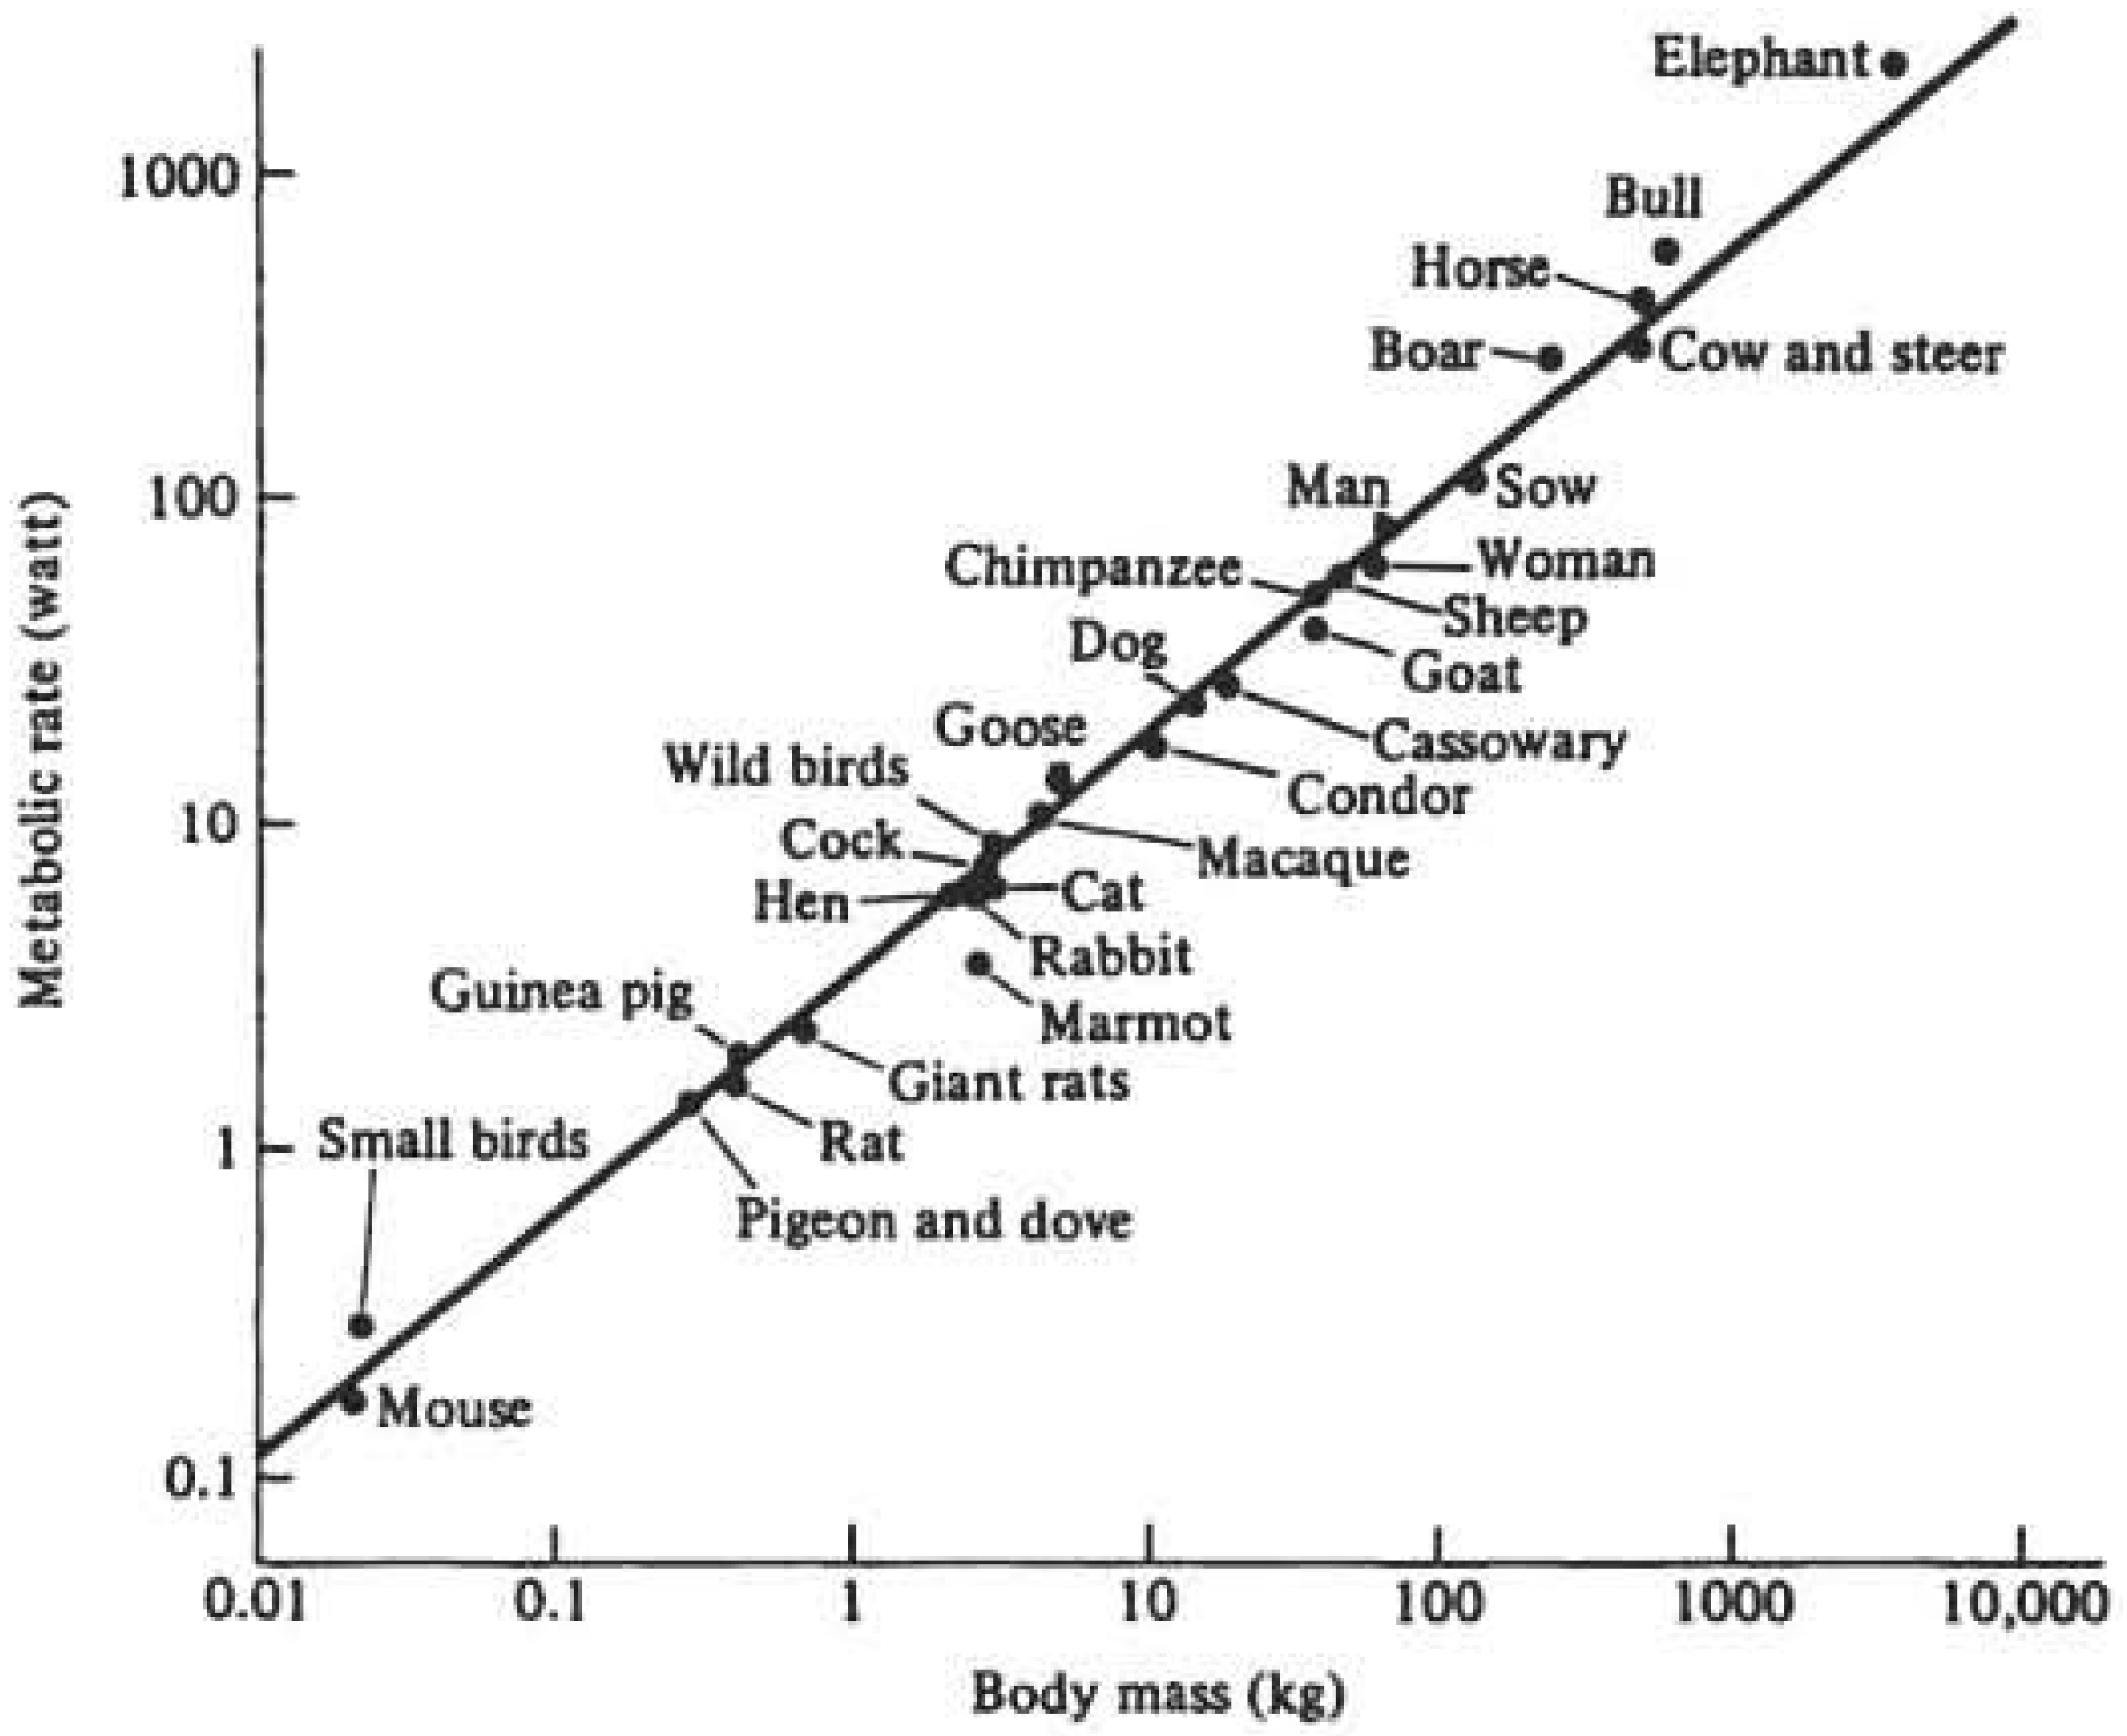
\includegraphics{images/systems-02-00089-g001.png}

  \begin{enumerate}

  \item

    \begin{grading}
      1 point
    \end{grading}

    \begin{problem}[0.25in]
      As you can probably guess, this is known as a \emph{log-log plot} since both axes use logarithmic scales. If we write $R$ for metabolic rate in watts and $M$ for body mass in kg, the vertical axis is really showing $\log_{10} R$, and the horizontal axis is really showing $\log_{10} M$. Label the axes. (That is, write the value of $\log_{10} R$ at each tick on the vertical axis and the value of $\log_{10} M$ at each tick on the horizontal axis.) 

      \begin{tikzpicture}[x=1.4cm, y=1.57cm]
        \draw (0, 0) node[anchor=south west] (image) { 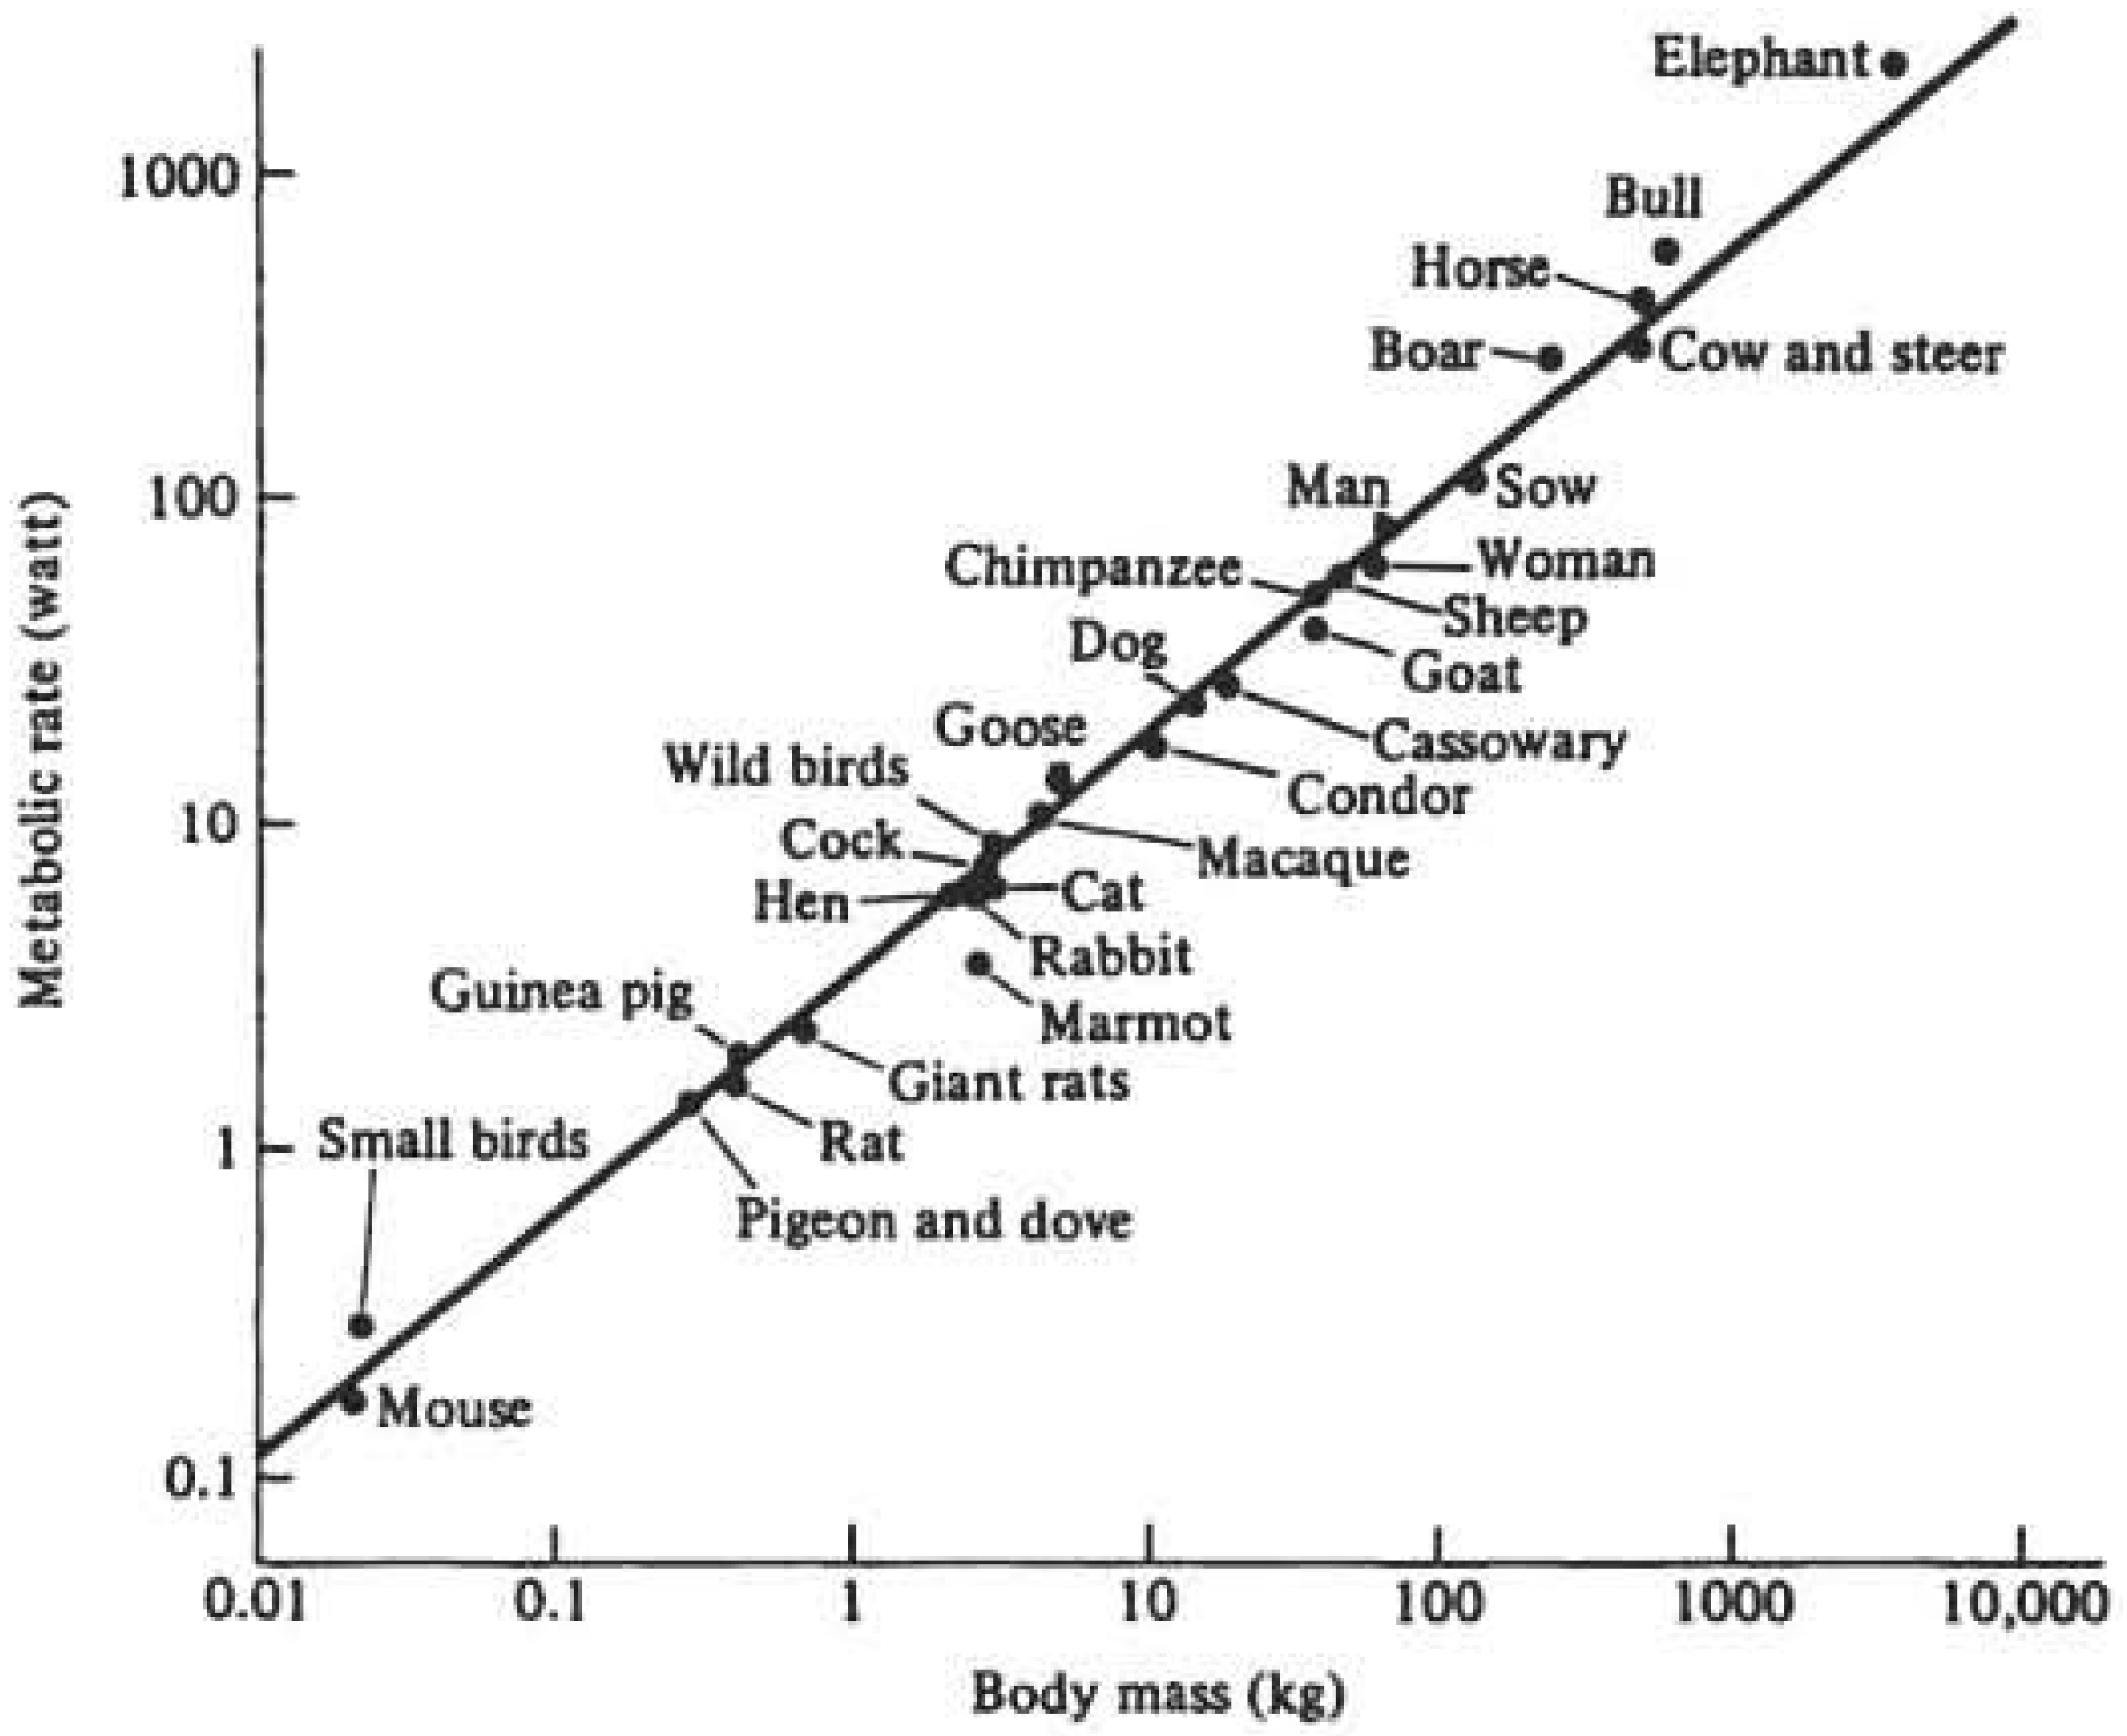
\includegraphics[trim=0.46in 0.3in 0 0, clip]{images/systems-02-00089-g001.png}}; %
        \draw (image.center |- 0, 0) node[below, yshift=-12pt] {$\log_{10} M$};
        \draw (0, 0 |- image.center) node[left, xshift=-18pt, yshift=18pt, rotate=90] {$\log_{10} R$};
        \solonly{%
          \begin{scope}[xshift=6pt]
            \draw (0, 0) node[below] { $-2$};%
            \draw (1, 0) node[below] {$-1$};%
            \draw (2, 0) node[below] {$0$};%
            \draw (3, 0) node[below] {$1$};%
            \draw (4, 0) node[below]{$2$};%
            \draw (5, 0) node[below]{$3$};%
            \draw (6, 0) node[below]{$4$};%
          \end{scope}
          \begin{scope}[yshift=16pt]
            \draw (0, 0) node[left]{$-1$};%
            \draw (0, 1) node[left]{$0$};%
            \draw (0, 2) node[left]{$1$};%
            \draw (0, 3) node[left]{$2$};%
            \draw (0, 4) node[left]{$3$};%
          \end{scope}
        }
      \end{tikzpicture}
    \end{problem}

    \pspace{\newpage}

  \item \label{mouse-to-elephant-fit}

    \begin{grading}
      1.5 points: 0.5 for the choice, 1 for the explanation
    \end{grading}

    \begin{problem}[\stretch{0.35}]
      One of the following is the equation of the line shown in the graph. Which one? How did you eliminate the other choices?
      \begin{enumerate}
      \item $\log_{10} R = 0.73 \log_{10} M - 0.91$
      \item $\log_{10} R = 0.73 \log_{10} M + 0.55$
      \item $\log_{10} R = -0.73 \log_{10} M - 0.91$
      \item $\log_{10} R = -0.73 \log_{10} M + 0.55$
      \end{enumerate}      
    \end{problem}

    \begin{solution}
      We know that the slope is positive, which eliminates
      choices (iii) and (iv). We also know that the $y$-intercept
      is positive, which eliminates choice (i). This only
      leaves \fbox{choice (ii)}.
    \end{solution}

  \item

    \begin{grading}
      2 points:
      \begin{itemize}[nosep]
      \item 0.5 for knowing $R = 10^{\log_{10} R}$
      \item 0.5 for knowing $10^{0.73 \log_{10} M +0.55 } = 10^{0.73 \log_{10} M} 10^{0.55}$
      \item 1 for knowing $10^{0.73 \log_{10} M} = M^{0.55}$
      \end{itemize}
    \end{grading}

    \begin{problem}[\vfill]
      Using the choice you picked in \ref{mouse-to-elephant-fit}, express the metabolic rate $R$ as a function of body mass $M$. Simplify your answer so that there are no logarithms left. 
    \end{problem}

    \begin{solution}
      \begin{align*}
        \log_{10} R &= 0.73 \log_{10} M +0.55  \\
        10^{\log_{10} R} &= 10^{0.73 \log_{10} M +0.55} \\
        R &= 10^{0.55}10^{0.73 \log_{10} M} \\
        R &= 10^{0.55} M^{0.73}
      \end{align*}
      So as a function of mass, \fbox{$R=10^{0.55}M^{0.73}$}.
    \end{solution}

  \item

    \begin{grading}
      0.5 points
    \end{grading}

    \begin{problem}[\vfill]
      Use \href{https://www.desmos.com/calculator}{Desmos} or some other tool to graph $R$ as a function of $M$, and sketch the graph. 
    \end{problem}

    \begin{solution}
      \begin{center}
        \begin{tikzpicture}
          \begin{axis}
            \addplot[domain=0:10000] {10^(0.55)*x^(0.73)};
          \end{axis}
        \end{tikzpicture}
      \end{center}
    \end{solution}

  \item

    \begin{grading}
      1 point
    \end{grading}

    \begin{problem}[\newpage]
      {\bf Looking back at your work in this problem:} If a log-log plot of a function $f(x)$ is linear, which of the following describes the form that $f(x)$ has? (In each choice, $a$ and $b$ are constants.) 

      \begin{enumeratecols}{3}
      \item $f(x) = ax + b$
      \item $f(x) = ax^b$
      \item $f(x) = a \cdot b^x$
      \end{enumeratecols}

      No explanation is necessary. 
    \end{problem}

    \begin{solution}
      The function we found in part (c) matches only choice (ii),
      \fbox{$f(x)=ax^b$}. We can show that this must be the
      case.
      \begin{align*}
          \log_{10} y &= m\log_{10}x + c \\
          10^{\log_{10}y} &= 10^{m\log_{10} x + c} \\
          y &= 10^c x^m
      \end{align*}
    \end{solution}

  \end{enumerate}

\item 
  % data from https://digfir-published.macmillanusa.com/psbe4e/psbe4e_ch13_8.html

  \note{Here's an increasing concave up function that isn't exponential.} 

  Here is \href{https://www.desmos.com/calculator/crrpolwdxo}{data showing the number of LinkedIn members between 2009 and 2014}. The independent variable is time in years, with $t = 0$ representing the first quarter of 2009; the dependent variable is the number of millions of LinkedIn members at that time.

  \begin{enumerate}
  \item

    \begin{grading}
      2 points: 0.5 for having a formula that goes through $(0, 37.3)$, 1.5 for having the rest of the formula
    \end{grading}

    \begin{problem}[\vfill]
      Let's try modeling this data with an exponential function. Find the exponential function that goes through the first and last data points, $(0, 37.3)$ and $(5.25, 313.4)$.
    \end{problem}

    \begin{solution}
      The value at $t=0$ is $37.3$, we would be multiplying by
      $\tfrac{313.4}{37.3}$ every $5.25$ years, so
      $f(t)=\boxed{37.3(\tfrac{313.4}{37.3})^{t/5.25}}$.
    \end{solution}

  \item

    \begin{grading}
      0.5 points
    \end{grading}

    \begin{problem}[\stretch{0.3}]
      Plot your exponential function with the data. Does it seem like a good match for the data?
    \end{problem}

    \begin{solution}
      No, the graph doesn't closely follow the data points.
    \end{solution}

  \calcitem \label{linkedin-percent-change-1}

    \begin{grading}
      0.5 points
    \end{grading}

    \begin{problem}[\stretch{0.3}]
      Find the percent change in the number of LinkedIn users between the first quarter of 2009 ($t = 0$) and the first quarter of 2010 ($t = 1$). 
    \end{problem}

    \begin{solution}
      The percent change from $t=0$ to $t=1$ is
      \begin{align*}
        \frac{64.2-37.3}{37.3} &\approx 0.72 \\
        &\approx \boxed{72\%}
      \end{align*}
    \end{solution}

  \calcitem \label{linkedin-percent-change-2}

    \begin{grading}
      0.5 points
    \end{grading}

    \begin{problem}[\stretch{0.3}]
      Find the percent change in the number of LinkedIn users between the first quarter of 2013 ($t = 4$) and the first quarter of 2014 ($t = 5$). 
    \end{problem}

    \begin{solution}
      The percent change from $t=4$ to $t=5$ is
      \begin{align*}
        \frac{296.5-218.3}{218.3} &\approx 0.36 \\
        &\approx \boxed{36\%}
      \end{align*}
    \end{solution}

  \item

    \begin{grading}
      1 point
    \end{grading}

    \begin{problem}[\nstretch{0.3}]
      Do your answers to \ref{linkedin-percent-change-1}  and \ref{linkedin-percent-change-2} suggest that the number of LinkedIn users was growing exponentially between 2009 and 2014? Explain. 
    \end{problem}

    \begin{solution}
      The answers to part (c) and (d) suggest that the number of LinkedIn
      users was \textbf{not} growing exponentially between 2009
      and 2014, because the yearly percent change was not constant.
    \end{solution}

    % No, yearly percent change isn't constant.

  \end{enumerate}

\calcitem % based on 13.3.45

  \begin{enumerate}

  \item

    \begin{grading}
      3 points: 1 for the equation for how much money there is at time $t$ (they might pick a particular starting amount of money, which is fine), 0.5 for setting up an equation to represent money increasing by 50\%, 1 for solving that equation exactly, 0.5 for the decimal approximation. 
    \end{grading}

    \begin{problem}[\vfill]
      Suppose you deposit some money in a bank account that earns a nominal annual interest rate of 3\%, compounded monthly. (See Example 9.7 in \href{https://canvas.harvard.edu/files/20608911/download?download_frd=1}{Gottlieb} or {{\#4}} on \href{https://canvas.harvard.edu/files/21231846/download?download_frd=1}{the worksheet ``Applications of Exponentials''} if you need a reminder of what this means.)

      If you make no deposits or withdrawals, how long will it take for the amount of money in the account to increase by 50\%? Please give both an exact answer and a decimal approximation. 
    \end{problem}

    \begin{solution}
      If we start with an amount of money $P$, then the amount $A$
      in an account earning $3\%$ nominal annual interest, compounded
      monthly, after $t$ years is
      \begin{align*}
        A &= P\Bigl(1+\frac{0.03}{12}\Bigr)^{12t} \\
        &= P(1.0025)^{12t}
      \end{align*}
      We want to determine the value of $t$ for which $A=1.5P$.
      \begin{align*}
        1.5P &= P(1.0025)^{12t} \\
        1.5 &= (1.0025)^{12t} \\
        12 t &= \log_{1.0025} 1.5 \\
        t &= \frac{1}{12} \log_{1.0025} 1.5 \\
        &= \frac{\ln 1.5}{12\ln 1.0025}
      \end{align*}
      So it will take $\boxed{\frac{\ln 1.5}{12\ln 1.0025}}$ or
      approximately $\boxed{13.5}$ years for the amount of money
      in the account to increase by 50\%.
    \end{solution}

  \item

    \begin{grading}
      3.5 points: 2 for setting up a correct equation to solve, 1 for correctly solving it, 0.5 for the decimal approximation
    \end{grading}

    \begin{problem}[\vfill\newpage]
      What would the annual interest rate need to be in order for your money to double in exactly 8 years (still assuming it's compounded monthly)? Again, give both an exact answer and a decimal approximation. 
    \end{problem}

    \begin{solution}  
      Let's call the nominal annual interest rate the account earns $r$.
      If we start with an amount $P$ and compound monthly, then
      the amount $A$ in the account after $8$ years is
      \[A=P\Bigl(1+\frac{r}{12}\Bigr)^{12\times 8}\]
      We want to determine the value of $r$ for which $A=2P$.
      \begin{align*}
        2P &= P\Bigl(1+\frac{r}{12}\Bigr)^{12 \times 8} \\
        2 &= \Bigl(1+\frac{r}{12}\Bigr)^{96} \\
        2^{1/96} &= 1+\frac{r}{12} \\
        2^{1/96} - 1 &= \frac{r}{12} \\
        12(2^{1/96}-1) &= r
      \end{align*}
      So the nominal annual interest rate needed is
      $\boxed{12(2^{1/96}-1)}$ or approximately $8.7\%$.
    \end{solution}

  \end{enumerate}

\item On January 1 of this year, Barry invested \$1000 in an account that promises to double his money every 10 years. On the same day, Charlotte invested \$800 in an account that promises to increase her money by 10\% each year. Suppose both accounts fulfill their promises. 

  \begin{enumerate}
  \item

    \begin{grading}
      2 points:
      \begin{itemize}[nosep]
      \item 0.5 for having the money at time 0 be 1000
      \item 0.5 for having $2^{\text{something}}$
      \item 1 for having $t / 10$ in the exponent
      \end{itemize}
    \end{grading}

    \begin{problem}[\stretch{0.5}]
      Write a formula for the amount of money Barry has $t$ years after investing. 
    \end{problem}

    \begin{solution}
      Barry starts with \$1000 at $t=0$ and the amount
      will be multiplied by 2 every 10 years, so 
      $B(t)=\boxed{1000(2)^{t/10}}$.
    \end{solution}

  \item

    \begin{grading}
      1 point
    \end{grading}

    \begin{problem}[\stretch{0.5}]
      Write a formula for the amount of money Charlotte has $t$ years after investing. 
    \end{problem}

    \begin{solution}
      Charlotte starts with \$800 dollars and the amount will be
      multiplied by 1.1 every year, so $C(t)=\boxed{800(1.1)^t}$.
    \end{solution}

  \calcitem

    \begin{grading}
      4 points: There are multiple ways to solve it; here's a breakdown for one likely method.
      \begin{itemize}[nosep]
      \item 0.5 for taking $\ln$ of both sides 
      \item 2 for correctly simplifying $\ln$ of each side
      \item 1 for solving the resulting linear equation
      \item 0.5 for giving a decimal approximation
      \end{itemize}
    \end{grading}

    \begin{problem}[\vfill]
      How many years will it take for Barry and Charlotte's accounts to have the same amount of money? Give an exact answer and a decimal approximation. 
    \end{problem}

    \begin{solution}
      We want to find the value of $t$ for which $B(t) = C(t)$.
      \begin{align*}
        1000(2)^{t/10} &= 800(1.1)^t \\
        \ln(1000(2)^{t/10}) &= \ln(800(1.1)^t) \\
        \ln1000 + \ln(2^{t/10}) &= \ln800 + \ln(1.1^t) \\
        \ln1000 + 0.1t\ln2 &= \ln800 + t\ln1.1 \\
        \ln1000 - \ln800 &= t\ln1.1 - 0.1t\ln2 \\
        \ln1000 - \ln800 &= t(\ln1.1 - 0.1\ln2) \\
        \frac{\ln1000-\ln800}{\ln1.1-0.1\ln2} &= t
      \end{align*}
      So it will take $\boxed{\frac{\ln1000-\ln800}{\ln1.1-0.1\ln2}}$
      or approximately $\boxed{8.6}$ years for Barry's and Charlotte's 
      accounts to have the same amount of money.
    \end{solution}

  \item

    \begin{grading}
      1.5 points: 0.5 for the choice, 1 for the explanation. They can also talk about how, if an account increases by 10\% per year, then it should increase by more than $10 \cdot 10\%$ in 10 years.
    \end{grading}

    \begin{problem}[\nstretch{0.5}]
      Whose account as a higher annual percent increase? How do you know? 
    \end{problem}

    \begin{solution}
      Since Charlotte started with less money but eventually catches up, she must have the higher annual percent increase. 
    \end{solution}

  \end{enumerate}
  
\item 
\label{graph-cubic-with-repeated-root}

  {\bf Preparation for next class}: In our next class, we'll be returning to polynomials and discussing some of the unique characteristics of their behavior. This problem is designed to review some of the core skills we use to analyze function behavior.

  Let $f(x) = (x - 1) (x + 3)^2$.

  \begin{enumerate}
  \item

    \begin{grading}
      1 point
    \end{grading}

    \begin{problem}[\vfill]
      Expand the formula for $f(x)$ to write it in the form $f(x) = ax^3 + bx^2 + cx + d$.
    \end{problem}

    \begin{solution}
      \begin{align*}
        f(x) &= (x-1)(x+3)^2 \\
        &= (x-1)(x^2 + 6x + 9) \\
        &= x^3 + 5x^2 + 3x - 9
      \end{align*}
    \end{solution}

  \item \label{graph-cubic-with-repeated-root-intercepts}

    \begin{grading}
      1 point, 0.5 for $x$-intercepts and 0.5 for $y$-intercept
    \end{grading}

    \begin{problem}[\vfill]
      What are the $x$- and $y$-intercepts of $y = f(x)$? 
    \end{problem}

    \begin{solution}
      The $x$-intercepts are $x=1$ and $x=-3$. The $y$-intercept
      is $y=-9$.
    \end{solution}

  \item \label{graph-cubic-with-repeated-root-increasing}

    \begin{grading}
      2.5 points:
      \begin{itemize}[nosep]
      \item 0.5 for calculating $f'(x)$ correctly
      \item 0.5 for solving $f'(x) = 0$ correctly
      \item 1 for testing the regions correctly
      \item 0.5 for a conclusion that's consistent with their sign chart
      \end{itemize}
    \end{grading}

    \begin{problem}[\nstretch{2}]
      Where is $f$ increasing? Where is $f$ decreasing?
    \end{problem}

    \begin{solution}
      We need to determine the sign of $f'(x) = 3x^2 + 10x + 3$. First,
      we set $f'(x)=0$ and solve for $x$:
      \begin{align*}
        0 &= 3x^2 + 10x + 3 \\
        &= (3x+1)(x+3)
      \end{align*}
      So $x=-3$ and $x=-1/3$. Since $y=f'(x)$ is an upward opening
      parabola, $f'(x)$ is positive on $(-\infty, -3)$, negative
      on $(-3, -1/3)$, and positive on $(-1/3, \infty)$. This means
      $f$ is increasing on $(-\infty, -3)$ and $(-1/3, \infty)$ and
      decreasing on $(-3, -1/3)$.
    \end{solution}

  \item \label{graph-cubic-with-repeated-root-concavity}

    \begin{grading}
      2.5 points, same breakdown as in \ref{graph-cubic-with-repeated-root-increasing} but for $f''$
    \end{grading}

    \begin{problem}[\vfill]
      Where is $f$ concave up? Where is $f$ concave down?
    \end{problem}

    \begin{solution}
      We need to determine the sign of $f''(x)=6x+10$. We can see
      that $f''(x)=0$ when $x=-5/3$, and since $y=f''(x)$ is a line
      with positive slope, $f''(x)$ is negative when $x<-5/3$ and positive
      when $x>5/3$. So $f$ is concave down on $(-\infty, -5/3)$ 
      and concave up on $(-5/3, \infty)$.
    \end{solution}

  \item

    \begin{grading}
      0.5 points, graded for consistency with their answer to \ref{graph-cubic-with-repeated-root-increasing}
    \end{grading}

    \begin{problem}[\vfill]
      What are the turning points of $f$?
    \end{problem}

    \begin{solution}
      The turning points are $x=-3$ and $x=-1/3$.
    \end{solution}

  \item

    \begin{grading}
      0.5 points, graded for consistency with their answer to \ref{graph-cubic-with-repeated-root-concavity} 
    \end{grading}

    \begin{problem}[\vfill]
      What are the inflection points of $f$? 
    \end{problem}

    \begin{solution}
      There is an inflection point at $x=-5/3$.
    \end{solution}

  \item

    \begin{grading}
      3 points:
      \begin{itemize}[nosep]
      \item 1 for having intercepts consistent with their answer to \ref{graph-cubic-with-repeated-root-intercepts}
      \item 1 for being consistent with their answer to \ref{graph-cubic-with-repeated-root-increasing}
      \item 1 for being consistent with their answer to \ref{graph-cubic-with-repeated-root-concavity} 
      \end{itemize}
    \end{grading}

    \begin{problem}[\vfill\newpage]
      Sketch the graph of $f$. Label all intercepts and the $x$-values of any turning points and inflection points. 
    \end{problem}

    \begin{solution}
      \begin{center}
        \begin{tikzpicture}
          \begin{axis}[xtick={-3,-5/3,-1/3,1}, ytick={-9},
          xticklabels={$-3$,$-5/3$,$-1/3$,$1$}]
            \addplot[domain=-5:2] {(x-1)*(x+3)^2};
          \end{axis}
        \end{tikzpicture}
      \end{center}
    \end{solution}
  \end{enumerate}


\end{enumerate}
\psreflection{For next class, read \S 11.1 - 11.3.}
\end{document}
